\documentclass[a4paper,14pt,oneside,openany]{memoir}

\tolerance10000
\hbadness10000

%%% Задаем поля, отступы и межстрочный интервал %%%

\usepackage[left=30mm, right=10mm, top=20mm, bottom=20mm]{geometry} % Пакет geometry с аргументами для определения полей
\pagestyle{plain} % Убираем стандарные для данного класса верхние колонтитулы с заголовком текущей главы, оставляем только номер страницы снизу по центру
\parindent=1cm % Абзацный отступ 1.25 см, приблизительно равно пяти знакам, как по ГОСТ
\usepackage{indentfirst} % Добавляем отступ к первому абзацу
%\linespread{1.3} % Межстрочный интервал (наиболее близко к вордовскому полуторному) - тут вместо этого используется команда OnehalfSpacing*

%%% Задаем языковые параметры и шрифт %%%

\usepackage[english, russian]{babel}                % Настройки для русского языка как основного в тексте
\babelfont{rm}{Times New Roman}                     % TMR в качестве базового roman-щрифта

% !TeX TXS-program:compile = --shell-escape
\usepackage[outputdir=.build]{minted} % Programming language syntax highlight

%%% Задаем стиль заголовков и подзаголовков в тексте %%%

\setsecnumdepth{subsection} % Номера разделов считать до третьего уровня включительно, т.е. нумеруются только главы, секции, подсекции
\renewcommand*{\chapterheadstart}{} % Переопределяем команду, задающую отступ над заголовком, чтобы отступа не было
\renewcommand*{\printchaptername}{} % Переопределяем команду, печатающую слово "Глава", чтобы оно не печалось
%\renewcommand*{\printchapternum}{} % То же самое для номера главы - тут не надо, номер главы оставляем
\renewcommand*{\chapnumfont}{\normalfont\bfseries} % Меняем стиль шрифта для номера главы: нормальный размер, полужирный
\renewcommand*{\afterchapternum}{\hspace{1em}} % Меняем разделитель между номером главы и названием
\renewcommand*{\printchaptertitle}{\normalfont\bfseries\centering\MakeUppercase} % Меняем стиль написания для заголовка главы: нормальный размер, полужирный, центрированный, заглавными буквами
\setbeforesecskip{20pt} % Задаем отступ перед заголовком секции
\setaftersecskip{20pt} % Ставим такой же отступ после заголовка секции
\setsecheadstyle{\raggedright\normalfont\bfseries} % Меняем стиль написания для заголовка секции: выравнивание по правому краю без переносов, нормальный размер, полужирный
\setbeforesubsecskip{20pt} % Задаем отступ перед заголовком подсекции
\setaftersubsecskip{20pt} % Ставим такой же отступ после заголовка подсекции
\setsubsecheadstyle{\raggedright\normalfont\bfseries}  % Меняем стиль написания для заголовка подсекции: выравнивание по правому краю без переносов, нормальный размер, полужирный

%%% Задаем параметры оглавления %%%

\addto\captionsrussian{\renewcommand\contentsname{Содержание}} % Меняем слово "Оглавление" на "Содержание"
\setrmarg{2.55em plus1fil} % Запрещаем переносы слов в оглавлении
%\setlength{\cftbeforechapterskip}{0pt} % Эта команда убирает интервал между заголовками глав - тут не надо, так красивее смотрится
\renewcommand{\aftertoctitle}{\afterchaptertitle \vspace{-\cftbeforechapterskip}} % Делаем отступ между словом "Содержание" и первой строкой таким же, как у заголовков глав
\renewcommand*{\chapternumberline}[1]{} % Делаем так, чтобы номер главы не печатался - тут не надо
\renewcommand*{\cftchapternumwidth}{1.5em} % Ставим подходящий по размеру разделитель между номером главы и самим заголовком
\renewcommand*{\cftchapterfont}{\normalfont\MakeUppercase} % Названия глав обычным шрифтом заглавными буквами
\renewcommand*{\cftchapterpagefont}{\normalfont} % Номера страниц обычным шрифтом
\renewcommand*{\cftchapterdotsep}{\cftdotsep} % Делаем точки до номера страницы после названий глав
\renewcommand*{\cftdotsep}{1} % Задаем расстояние между точками
\renewcommand*{\cftchapterleader}{\cftdotfill{\cftchapterdotsep}} % Делаем точки стандартной формы (по умолчанию они "жирные")
\renewcommand*{\baselinestretch}{1.5} % Межстрочный интервал 
\maxtocdepth{subsection} % В оглавление попадают только разделы первыхтрех уровней: главы, секции и подсекции

%%% Выравнивание и переносы %%%

%% http://tex.stackexchange.com/questions/241343/what-is-the-meaning-of-fussy-sloppy-emergencystretch-tolerance-hbadness
%% http://www.latex-community.org/forum/viewtopic.php?p=70342#p70342
\tolerance 1414
\hbadness 1414
\emergencystretch 1.5em                             % В случае проблем регулировать в первую очередь
\hfuzz 0.3pt
\vfuzz \hfuzz
%\dbottom
%\sloppy                                            % Избавляемся от переполнений
\clubpenalty=10000                                  % Запрещаем разрыв страницы после первой строки абзаца
\widowpenalty=10000                                 % Запрещаем разрыв страницы после последней строки абзаца
\brokenpenalty=4991                                 % Ограничение на разрыв страницы, если строка заканчивается переносом

%%% Объясняем компилятору, какие буквы русского алфавита можно использовать в перечислениях (подрисунках и нумерованных списках) %%%
%%% По ГОСТ нельзя использовать буквы ё, з, й, о, ч, ь, ы, ъ %%%
%%% Здесь также переопределены заглавные буквы, хотя в принципе они в документе не используются %%%

\makeatletter
    \def\russian@Alph#1{\ifcase#1\or
       А\or Б\or В\or Г\or Д\or Е\or Ж\or
       И\or К\or Л\or М\or Н\or
       П\or Р\or С\or Т\or У\or Ф\or Х\or
       Ц\or Ш\or Щ\or Э\or Ю\or Я\else\xpg@ill@value{#1}{russian@Alph}\fi}
    \def\russian@alph#1{\ifcase#1\or
       а\or б\or в\or г\or д\or е\or ж\or
       и\or к\or л\or м\or н\or
       п\or р\or с\or т\or у\or ф\or х\or
       ц\or ш\or щ\or э\or ю\or я\else\xpg@ill@value{#1}{russian@alph}\fi}
\makeatother

%%% Задаем параметры оформления рисунков и таблиц %%%

\usepackage{graphicx, caption, subcaption} % Подгружаем пакеты для работы с графикой и настройки подписей
\graphicspath{{src/}} % Определяем папку с рисунками
\captionsetup[figure]{font=small, width=\textwidth, name=Рисунок, justification=centering} % Задаем параметры подписей к рисункам: маленький шрифт (в данном случае 12pt), ширина равна ширине текста, полнотекстовая надпись "Рисунок", выравнивание по центру
% \captionsetup[subfigure]{font=small} % Индексы подрисунков а), б) и так далее тоже шрифтом 12pt (по умолчанию делает еще меньше)
\captionsetup[table]{singlelinecheck=false,font=small,width=\textwidth,justification=justified} % Задаем параметры подписей к таблицам: запрещаем переносы, маленький шрифт (в данном случае 12pt), ширина равна ширине текста, выравнивание по ширине
\captiondelim{ --- } % Разделителем между номером рисунка/таблицы и текстом в подписи является длинное тире
\setkeys{Gin}{width=\textwidth} % По умолчанию размер всех добавляемых рисунков будет подгоняться под ширину текста
\renewcommand{\thesubfigure}{\asbuk{subfigure}} % Нумерация подрисунков строчными буквами кириллицы
%\setlength{\abovecaptionskip}{0pt} % Отбивка над подписью - тут не меняем
%\setlength{\belowcaptionskip}{0pt} % Отбивка под подписью - тут не меняем
\usepackage[section]{placeins} % Объекты типа float (рисунки/таблицы) не вылезают за границы секциии, в которой они объявлены

%%% Задаем параметры ссылок и гиперссылок %%% 

\usepackage{hyperref}                               % Подгружаем нужный пакет
\hypersetup{
    colorlinks=true,                                % Все ссылки и гиперссылки цветные
    linktoc=all,                                    % В оглавлении ссылки подключатся для всех отображаемых уровней
    linktocpage=true,                               % Ссылка - только номер страницы, а не весь заголовок (так выглядит аккуратнее)
    linkcolor=black,                                  % Цвет ссылок и гиперссылок - красный
    citecolor=black                                   % Цвет цитировний - красный
}

%%% Настраиваем отображение списков %%%

\usepackage{enumitem}                               % Подгружаем пакет для гибкой настройки списков
\renewcommand*{\labelitemi}{\normalfont{--}}        % В ненумерованных списках для пунктов используем короткое тире
\makeatletter
    \AddEnumerateCounter{\asbuk}{\russian@alph}     % Объясняем пакету enumitem, как использовать asbuk
\makeatother
\renewcommand{\labelenumii}{\asbuk{enumii})}        % Кириллица для второго уровня нумерации
\renewcommand{\labelenumiii}{\arabic{enumiii})}     % Арабские цифры для третьего уровня нумерации
\setlist{noitemsep, leftmargin=*}                   % Убираем интервалы между пунками одного уровня в списке
\setlist[1]{labelindent=\parindent}                 % Отступ у пунктов списка равен абзацному отступу
\setlist[2]{leftmargin=\parindent}                  % Плюс еще один такой же отступ для следующего уровня
\setlist[3]{leftmargin=\parindent}                  % И еще один для третьего уровня

%%% Счетчики для нумерации объектов %%%

\counterwithout{figure}{chapter}                    % Сквозная нумерация рисунков по документу
\counterwithout{equation}{chapter}                  % Сквозная нумерация математических выражений по документу
\counterwithout{table}{chapter}                     % Сквозная нумерация таблиц по документу

%%% Реализация библиографии пакетами biblatex и biblatex-gost с использованием движка biber %%%

\usepackage{csquotes} % Пакет для оформления сложных блоков цитирования (biblatex рекомендует его подключать)
\usepackage[%
backend=biber,                                      % Движок
bibencoding=utf8,                                   % Кодировка bib-файла
sorting=none,                                       % Настройка сортировки списка литературы
style=gost-numeric,                                 % Стиль цитирования и библиографии по ГОСТ
language=auto,                                      % Язык для каждой библиографической записи задается отдельно
autolang=other,                                     % Поддержка многоязычной библиографии
sortcites=true,                                     % Если в квадратных скобках несколько ссылок, то отображаться будут отсортированно
movenames=false,                                    % Не перемещать имена, они всегда в начале библиографической записи
maxnames=5,                                         % Максимальное отображаемое число авторов
minnames=3,                                         % До скольки сокращать число авторов, если их больше максимума
doi=false,                                          % Не отображать ссылки на DOI
isbn=false,                                         % Не показывать ISBN, ISSN, ISRN
]{biblatex}[2016/09/17]
\DeclareDelimFormat{bibinitdelim}{}                 % Убираем пробел между инициалами (Иванов И.И. вместо Иванов И. И.)
\addbibresource{literature.bib}                     % Определяем файл с библиографией

%%% Скрипт, который автоматически подбирает язык (и, следовательно, формат) для каждой библиографической записи %%%
%%% Если в названии работы есть кириллица - меняем значение поля langid на russian %%%
%%% Все оставшиеся пустые места в поле langid заменяем на english %%%

% \DeclareSourcemap{
%   \maps[datatype=bibtex]{
%     \map{
%         \step[fieldsource=title, match=\regexp{^\P{Cyrillic}*\p{Cyrillic}.*}, final]
%         \step[fieldset=langid, fieldvalue={russian}]
%     }
%     \map{
%         \step[fieldset=langid, fieldvalue={english}]
%     }
%   }
% }

%%% Прочие пакеты для расширения функционала %%%

\usepackage{longtable,ltcaption}                    % Длинные таблицы
\usepackage{multirow,makecell}                      % Улучшенное форматирование таблиц
\usepackage{booktabs}                               % Еще один пакет для красивых таблиц
\usepackage{soul}                                   % Поддержка переносоустойчивых подчёркиваний и зачёркиваний
\usepackage{icomma}                                 % Запятая в десятичных дробях
\usepackage{hyphenat}                               % Для красивых переносов
\usepackage{textcomp}                               % Поддержка "сложных" печатных символов типа значков иены, копирайта и т.д.
\usepackage[version=4]{mhchem}                      % Красивые химические уравнения
\usepackage{amsmath}                                % Усовершенствование отображения математических выражений 

%%% Вставляем по очереди все содержательные части документа %%%

\begin{document}

\thispagestyle{empty}

\begin{center}
    МИНИСТЕРСТВО ОБРАЗОВАНИЯ РЕСПУБЛИКИ БЕЛАРУСЬ \\ 
    БЕЛОРУССКИЙ ГОСУДАРСТВЕННЫЙ УНИВЕРСИТЕТ \\ 
    ФИЗИЧЕСКИЙ ФАКУЛЬТЕТ \\
    Кафедра компьютерного моделирования
\end{center}

\vspace{100pt}

\begin{center}
    \textbf{ФИЗИЧЕСКИ-ИНФОРМИРОВАННЫЕ НЕЙРОННЫЕ СЕТИ ДЛЯ РЕШЕНИЯ ЗАДАЧ ГИДРОДИНАМИКИ}
    
    \hspace{10mm}
    \textbf{Курсовая работа}
    \hspace{10mm}
    
    Специальность 1-31 04 08 Компьютерная физика
\end{center}

\vfill

\begin{flushright}
    \textbf{Исполнитель:} \\
    студент III курса 4 группы \\
    Степанов Игорь Дмитриевич \\
    \vspace{10mm}    
    \textbf{Научный руководитель:} \\
    старший преподаватель \\
    Тимощенко Игорь Андреевич
\end{flushright}

\vfill

\begin{center}
    Минск, 2024
\end{center}                                     % Титульник

\newpage % Переходим на новую страницу
\setcounter{page}{2} % Начинаем считать номера страниц со второй
\OnehalfSpacing* % Задаем полуторный интервал текста (в титульнике одинарный, поэтому команда стоит после него)

\tableofcontents*                                   % Автособираемое оглавление

\newpage

\chapter{Введение}

Применение нейронных сетей стремительно набирает популярность во многих областях.
Нейросети активно используются широкими массами как в повседневной жизни, так и в
профессиональной деятельности. Их внедряют в голосовых ассистентов, распространенные
среды разработки, системы перевода, а также они выступают в роли самостоятельных
программ для генерации изображений или текста.

Нейронные сети представляют собой сложные вычислительные системы, внутреннее
функционирование которых трудно точно предсказать из-за их ''черного ящика''
(рис. \ref{fig:black_box}) природы. Они принимают на вход набор данных, которые
проходят через множество скрытых слоев, где происходят операции умножения на веса,
сложения и применения нелинейных функций в определенной последовательности.
Эти вычисления в итоге преобразуют входные данные в выходные значения требуемого
формата. В процессе обучения нейросети вычисляется ошибка между полученным выходом
и ожидаемым результатом на обучающих примерах. Затем используются оптимизационные 
алгоритмы для минимизации этой ошибки путем настройки весов внутри сети. 
Таким образом, сеть обучается выполнять желаемую задачу.

\begin{figure}[h]
    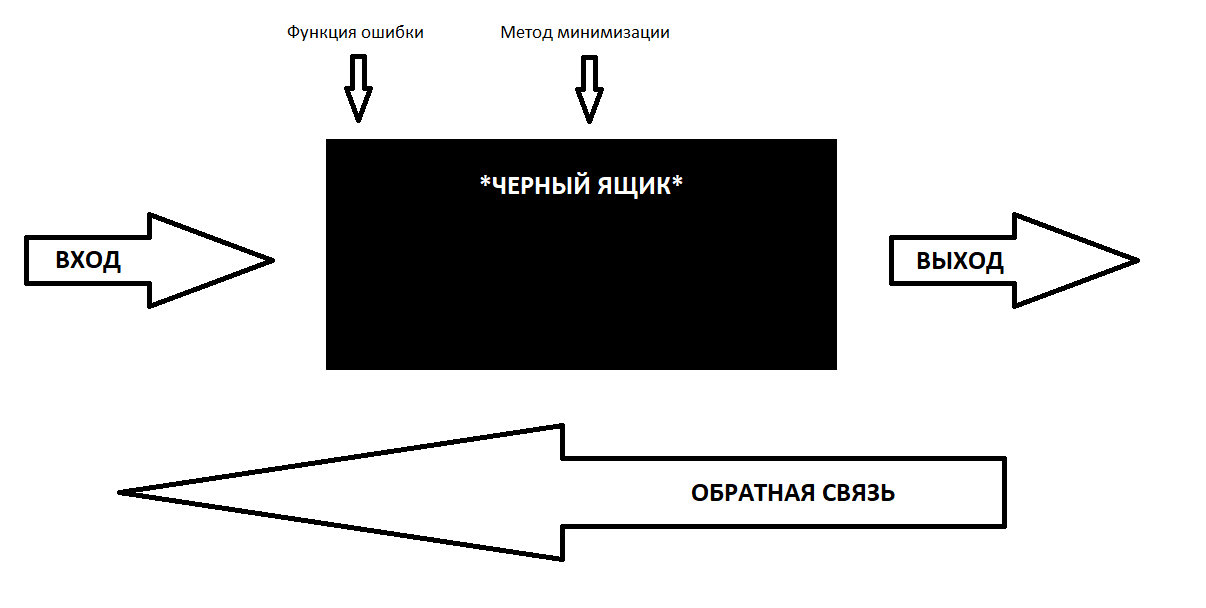
\includegraphics{introdution/black_box.png}
    \caption{Простейшее представление работы нейронной сети}
    \label{fig:black_box}
\end{figure}

Благодаря гибкости функции ошибки, нейронные сети можно использовать для решения
различных уравнений и задач. Функцию ошибки можно задать как невязку между желаемым
решением и выходом нейросети. Этот подход может быть эффективным, поскольку после
однократного обучения нейросеть становится моделью, способной быстро решать целое
семейство однотипных задач. Хотя сам процесс получения предсказаний от обученной
сети также требует вычислительных ресурсов, использование специализированных нейронных
процессоров (NPU) потенциально может ускорить этот процесс без необходимости сложных
оптимизаций и распараллеливания. Таким образом, после начальных затрат на обучение,
нейросеть превращается в эффективный инструмент для быстрого решения множества сходных
задач вычислительного характера.

P.S.: Написано нейронной сетью Claude-3-Sonnet
% \chapter{Цели}
\begin{enumerate}
    \item Изучить возможности работы с NPU на телефонах нового поколения.
    \item Сделать методическое пособие для работы с библиотекой \textbf{DeepXDE} \cite{lu2021deepxde}.
    \item Рассмотреть нейронные сети как метод решения дифферинциальных уравнений второго порядка
    для гидродинамики.
    \item Предложить применение данного механизма в будущем.
\end{enumerate}

\chapter{Задачи}
\begin{enumerate}
    \item Изучить материал по работе с NPU \cite{nnapi}.
    \item Описать базовый функционал \textbf{DeepXDE}.
    \item Написать код с использованием библиотеки \textbf{DeepXDE} для решения нескольких 
    показательных задач из области гидродинамики.
\end{enumerate}

\chapter{Обзор библиотеки DeepXDE \cite{lu2021deepxde}}

DeepXDE (Deep Learning for Differential Equations) –-- это открытая библиотека для Python,
предназначенная для решения различных типов дифференциальных уравнений с помощью методов
глубокого обучения. Она была разработана группой исследователей из Научно-технического
университета Китая и представлена в 2019 году. DeepXDE позволяет решать задачи, описываемые
обыкновенными и частными дифференциальными уравнениями, включая уравнения в частных производных,
интегро-дифференциальные уравнения и уравнения с переменными коэффициентами.

Данная библиотека поддерживает следущие крупные библиотеки машинного обучения: tensorflow.compat.v1,
tensorflow, pytorch, jax, paddle.

\section{Возможности библиотеки}
Для постановки физической задачи необходимо четко определить, что рассматривается в качестве системы
(тело, частица, сплошная среда и т.д.), а также ее границы и взаимодействие с окружающей средой.
Следует задать начальное состояние системы, такое как начальное положение, скорость, температура,
давление и т.д. Необходимо определить, какие физические законы и принципы применимы к данной системе
(законы Ньютона, законы сохранения, принципы термодинамики и т.д.), и записать уравнения, описывающие
движение, взаимодействие или другие процессы в системе, на основе выбранных законов и принципов. При
необходимости нужно задать дополнительные условия, такие как связи, граничные условия, свойства
материалов и т.д. Также следует четко сформулировать, какие физические величины необходимо определить
в результате решения задачи. Этот минимум информации позволяет корректно сформулировать физическую
задачу и создать математическую модель для ее решения.

Суть метода заключается в использовании невязки всех уравнений, граничных и начальных условий в качестве
функции потерь. Это позволяет нейронной сети минимизировать данную ошибку и получить необходимый результат.

Невязка - это разница между левым и правым значениями уравнений. Она рассчитывается на основе начального решения,
которое задается случайным образом. Затем, с помощью методов минимизации функции потерь, решение уточняется.

Аналогичный метод решения мы можем видеть при численном решении системы линейных алгебраических уравнений (СЛАУ)
с помощью градиентного спуска. В этом случае, невязка также используется в качестве функции потерь, но минимизирует
ее Градиентный спуск, чтобы получить решение СЛАУ.

Градиентный спуск - это один из наиболее распространенных методов минимизации функции потерь. Он заключается в том,
что на каждом шаге алгоритма мы изменяем решение в направлении, которое уменьшает значение функции потерь.

\subsection{Область}
Библиотека DeepXDE имеет ряд стандартных областей (geometry), которые можно применить к большинству задач:
\begin{minted}{python}
from deepxde.geometry.geometry_1d import Interval
from deepxde.geometry.geometry_2d import (
    Disk, Ellipse, Polygon, Rectangle, StarShaped, Triangle
)
from deepxde.geometry.geometry_3d import Cuboid, Sphere
from deepxde.geometry.geometry_nd import Hypercube, Hypersphere
from deepxde.geometry.timedomain  import GeometryXTime, TimeDomain
\end{minted}
Объекты данных классов имеют следущий функционал (весь функционал унаследован от интерфейсного класса deepxde.geometry.Geometry):
\begin{itemize}
    \item Проверить, принадлежит ли точка данной области или ее границе
    \item Нормаль к границе.
    \item Объединение, пересечение и интерсекцию с другими обдостями.
    \item Получить набор случайных точек в данной области или на ее границе.
\end{itemize}
Эти возможности предоставляют полный доступ к созданию и использованию области для решения
дифференциальных уравнений.

Например для рассмотрения обтекания бесконечного цилиндра нам потребуется следущая область:
\begin{minted}{python}
base_domain = Rectangle(xmin=[0, 0], xmax=[3, 1])
barrier_domain = Ellipse(
    center=[0.5, 0.5], semimajor=0.1, semiminor=0.1
    )
space_domain = base_domain - barrier_domain

time_domain = dde.geometry.TimeDomain(0, 1)

domain = dde.geometry.GeometryXTime(space_domain, time_domain)
\end{minted}
Далее мы будем использовать данную область для примера решенния задачи.
\subsection{Уравнения}
Для задания уравнения или системы уравнений мы можем использовать следущие два оператора:
\begin{minted}{python}
deepxde.grad.jacobian
deepxde.grad.hessian
\end{minted}
Они представляют собой операторы набла и Лапласа соответственно. Для использования уравнений
в дальнейшем необходимо создать функцию, которая будет возвращать уравнение или массив уравнений.

Для задач гидродинамики воспользуемся уравнения Навье-Стокса. Пример реализации уравнений
для двумерной задачи:
\begin{minted}{python}
def navier_stocks(x, u):
    u_vel, v_vel, p = u[:, 0:1], u[:, 1:2], u[:, 2:3]

    u_vel_x = dde.grad.jacobian(u, x, i=0, j=0)
    u_vel_y = dde.grad.jacobian(u, x, i=0, j=1)
    u_vel_t = dde.grad.jacobian(u, x, i=0, j=2)
    u_vel_xx = dde.grad.hessian(u, x, component=0, i=0, j=0)
    u_vel_yy = dde.grad.hessian(u, x, component=0, i=1, j=1)

    v_vel_x = dde.grad.jacobian(u, x, i=1, j=0)
    v_vel_y = dde.grad.jacobian(u, x, i=1, j=1)
    v_vel_t = dde.grad.jacobian(u, x, i=1, j=2)
    v_vel_xx = dde.grad.hessian(u, x, component=1, i=0, j=0)
    v_vel_yy = dde.grad.hessian(u, x, component=1, i=1, j=1)

    p_x = dde.grad.jacobian(u, x, i=2, j=0)
    p_y = dde.grad.jacobian(u, x, i=2, j=1)

    momentum_x = (
        u_vel_t
        + (u_vel * u_vel_x + v_vel * u_vel_y)
        + p_x
        - 1 / Re * (u_vel_xx + u_vel_yy)
    )
    momentum_y = (
        v_vel_t
        + (u_vel * v_vel_x + v_vel * v_vel_y)
        + p_y
        - 1 / Re * (v_vel_xx + v_vel_yy)
    )
    continuity = u_vel_x + v_vel_y
    return [momentum_x, momentum_y, continuity]
\end{minted}

\subsection{Граничные и начальные условия}
Для задания граничных условий используются следущие классы в DeepXDE (подпространство deepxde\.icbc):
\begin{itemize}
\item DirichletBC
\item NeumannBC
\item OperatorBC
\item RobinBC
\item PeriodicBC
\item PointSetBC
\item PointSetOperatorBC
\end{itemize}

Каждый из них задает соответствующее условие, а также позволяет унаследовать и изменить условия
для определения границы с помощью вспомогательного аргумента.

Для начальных условий из того же подпространства есть класс IC, который задает значение нашего решения в начальный
момент времени и также, как и граничные условия, может переопределять условия для границы.

Пример реализации условий для уравнения Навье-Стокса в двумерной задаче:
\begin{minted}{python}
boundary_condition_u = dde.DirichletBC(
    domain, lambda x: 1, 
    lambda x, on_boundary: base_domain.on_boundary(x[0:2]),
    component=0
)
boundary_condition_v = dde.DirichletBC(
    domain, lambda x: 0, 
    lambda x, on_boundary: base_domain.on_boundary(x[0:2]),
    component=1
)
barrier_condition_u = dde.DirichletBC(
    domain, lambda x: 0, 
    lambda x, on_boundary: barrier_domain.on_boundary(x[0:2]),
    component=0
)
barrier_condition_v = dde.DirichletBC(
    domain, lambda x: 0, 
    lambda x, on_boundary: barrier_domain.on_boundary(x[0:2]),
    component=1
)

initial_condition_u = dde.IC(
    domain, lambda x: 0,
    lambda x, on_initial: on_initial,
    component=0
)
initial_condition_v = dde.IC(
    domain, lambda x: 0,
    lambda x, on_initial: on_initial, 
    component=1
)
\end{minted}
    
\subsection{Создание модели}
Пример:
\begin{minted}{python}
data = dde.data.TimePDE(
    domain,
    navier_stocks,
    [
        boundary_condition_u,
        boundary_condition_v,
        initial_condition_u,
        initial_condition_v,
        barrier_condition_u,
        barrier_condition_v,
    ],
    num_domain=50000,
    num_boundary=5000,
    num_initial=5000,
    num_test=10000,
)

net = dde.nn.FNN([3] + 4 * [50] + [3], "tanh", "Glorot normal")

model = dde.Model(data, net)    
\end{minted}
\subsection{Обучение модели}
Пример:
\begin{minted}{python}
model.compile("adam", lr=1e-3, loss_weights=[1, 1, 100, 10, 10, 10, 10, 10, 10])
model.train(iterations=3000, display_every=1)
model.compile("L-BFGS", loss_weights=[1, 1, 100, 10, 10, 10, 10, 10, 10])
losshistory, train_state = model.train()
\end{minted}
Также имеется возможность сохранять и загружать существующую модель:
\begin{minted}{python}
model.train(iterations=3000, display_every=1, model_save_path="model/")

model.restore("model/good_model.ckpt-43904.ckpt", verbose=1)    
\end{minted}
\subsection{Применение модели}
Для создания модели требуется четкое понимание функции ошибки и оптимизаторов, способных минимизировать данную функцию.
Так как мы не можем гарантированно знать нашу функцию ошибки, остается только эксперементировать с различными
оптимизаторами.

В данной библиотеке доступны все оптимизаторы из соответствующей оболочки для нейронных сетей. В данной работе преимущественно
используется Tensorflow, поэтому доступны следущие оптимизаторы

\begin{itemize}
    \item Adadelta
    \item Adafactor
    \item Adagrad
    \item Adam
    \item AdamW
    \item Adamax
    \item Ftrl
    \item Lion
    \item Nadam
    \item RMSprop
    \item SGD
\end{itemize}
А также L-BFGS и L-BFGS-B предоставляемые самой библиотекой DeepXDE.
Для остальных доступных оболочек соответствующие им оптимизаторы можно найти тут tensorflow.compat.v1 \cite{tfv1opt},
tensorflow \cite{tfopt}, pytorch \cite{pytorchopt}, jax \cite{jaxopt}, paddle \cite{paddleopt}.

Далее нужно оценить весовые коэффициенты для каждого из входных условий. Например, в последущих примерах я отдаю предпочтение
выполнению граничных условий, поэтому они идут с весом 100, и уравнение непрерывности с весом 10, остальное 1.



\chapter{Использование NPU для ускорения работы модели}

С точки зрения возможности использования NPU следует выбирать tensorflow или tensorflow.compat.v1,
так как они поддерживают экспорт модели в TensorFlow Lite и их использование на устройствах Android
и iOS\cite{nnapi}. Такой подход можно использовать для реалистичного моделирования физики как в научных целях, так и
в мобильных играх.

Для реализации приложения с такими возм

\printbibliography[title=Список использованных источников] % Автособираемый список литературы


\end{document}